\documentclass[11pt]{beamer}
\usepackage[utf8]{inputenc}
\usepackage[T1]{fontenc}
\usepackage{lmodern}
\usepackage{amsmath}
\usepackage{amsfonts}
\usepackage{amssymb}
\usepackage{graphicx}
\usepackage{ragged2e}
\usepackage{enumitem}
\usepackage[spanish]{babel}
\usetheme{Madrid}

\author{Alina María de la Noval Armenteros}
\title{Presentación del Moogle en \LaTeX}
\subtitle{Manual de Uso y de Programación}
\logo{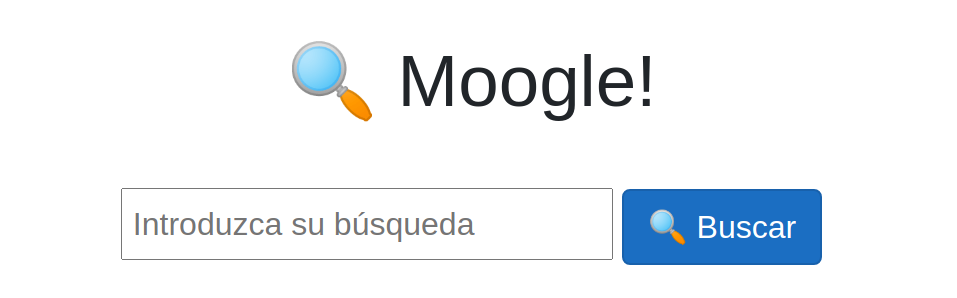
\includegraphics[scale=0.12]{moogle.png}}
\institute[UH]{Facultad de Matemática y Computación\\Universidad de la Habana}
\date{19 de julio de 2023}
  
  
\AtBeginSection[]
{
	\begin{frame}<beamer>{Contenido}
		\tableofcontents[currentsection]
\end{frame}
}

\begin{document}
	
	\begin{frame}
		\maketitle
	\end{frame}
	
	\begin{frame}{Contenido}
		\tableofcontents
	\end{frame}
	
	\section {¿Cómo trabajar con esta aplicación?}
	\begin{frame}{¿Cómo trabajar con esta aplicación?} 
		\justifying
		\large Al ejecutar el proyecto, aparece en pantalla una página con la siguiente imagen:
		
		\begin{figure}[H]
			\centering
			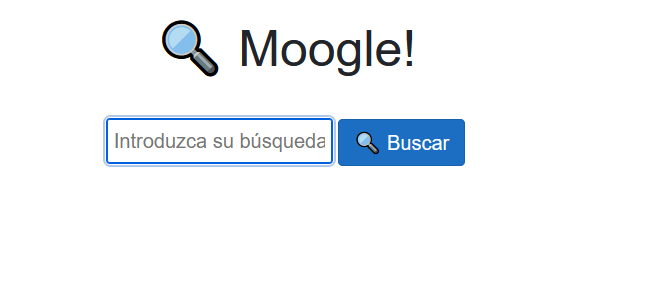
\includegraphics[scale=0.5]{img.png}
			\caption{Página principal del Moogle}
			\label{fig: Figura 1}
		\end{figure}
		
	\end{frame}
	
	\begin{frame}{¿Cómo trabajar con esta aplicación?}
		\justifying
		Para comenzar a realizar las búsquedas se debe teclear en el cuadro de texto la consulta que se desea buscar si existe en alguno de los archivos que se tienen a disposición.\\
		
		Luego de entrar el texto a buscar se debe dar con el click del mouse en el botón Buscar para que el sistema ejecute la búsqueda.
		
		\begin{figure}[H]
			\centering
			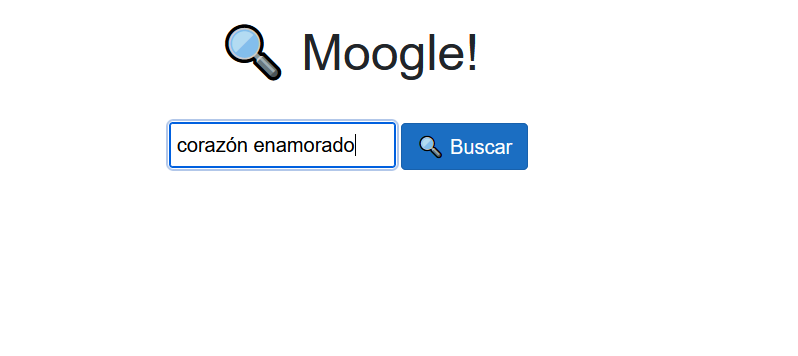
\includegraphics[scale=0.5]{img2.png}
			\caption{Proceso de búsqueda del documento}
			\label{fig: Figura 2}
		\end{figure}
	\end{frame}
	
	\begin{frame}{¿Cómo trabajar con esta aplicación?}
		\justifying
		Luego de unos segundos se muestra en el extremo derecho el listado de los ficheros que contienen las palabras que se entraron en el texto de búsqueda. Estos ficheros se muestran descendentemente según el peso de las palabras buscadas en los ficheros predefinidos. Se mostrarán siempre los cinco primeros ficheros.\\
		
		Debajo del nombre del fichero se muestra un fragmento del fichero donde se encuentra el texto buscado.
	\end{frame}
	
	\begin{frame}{¿Cómo trabajar con esta aplicación?}
		\begin{figure}[H]
			\centering
			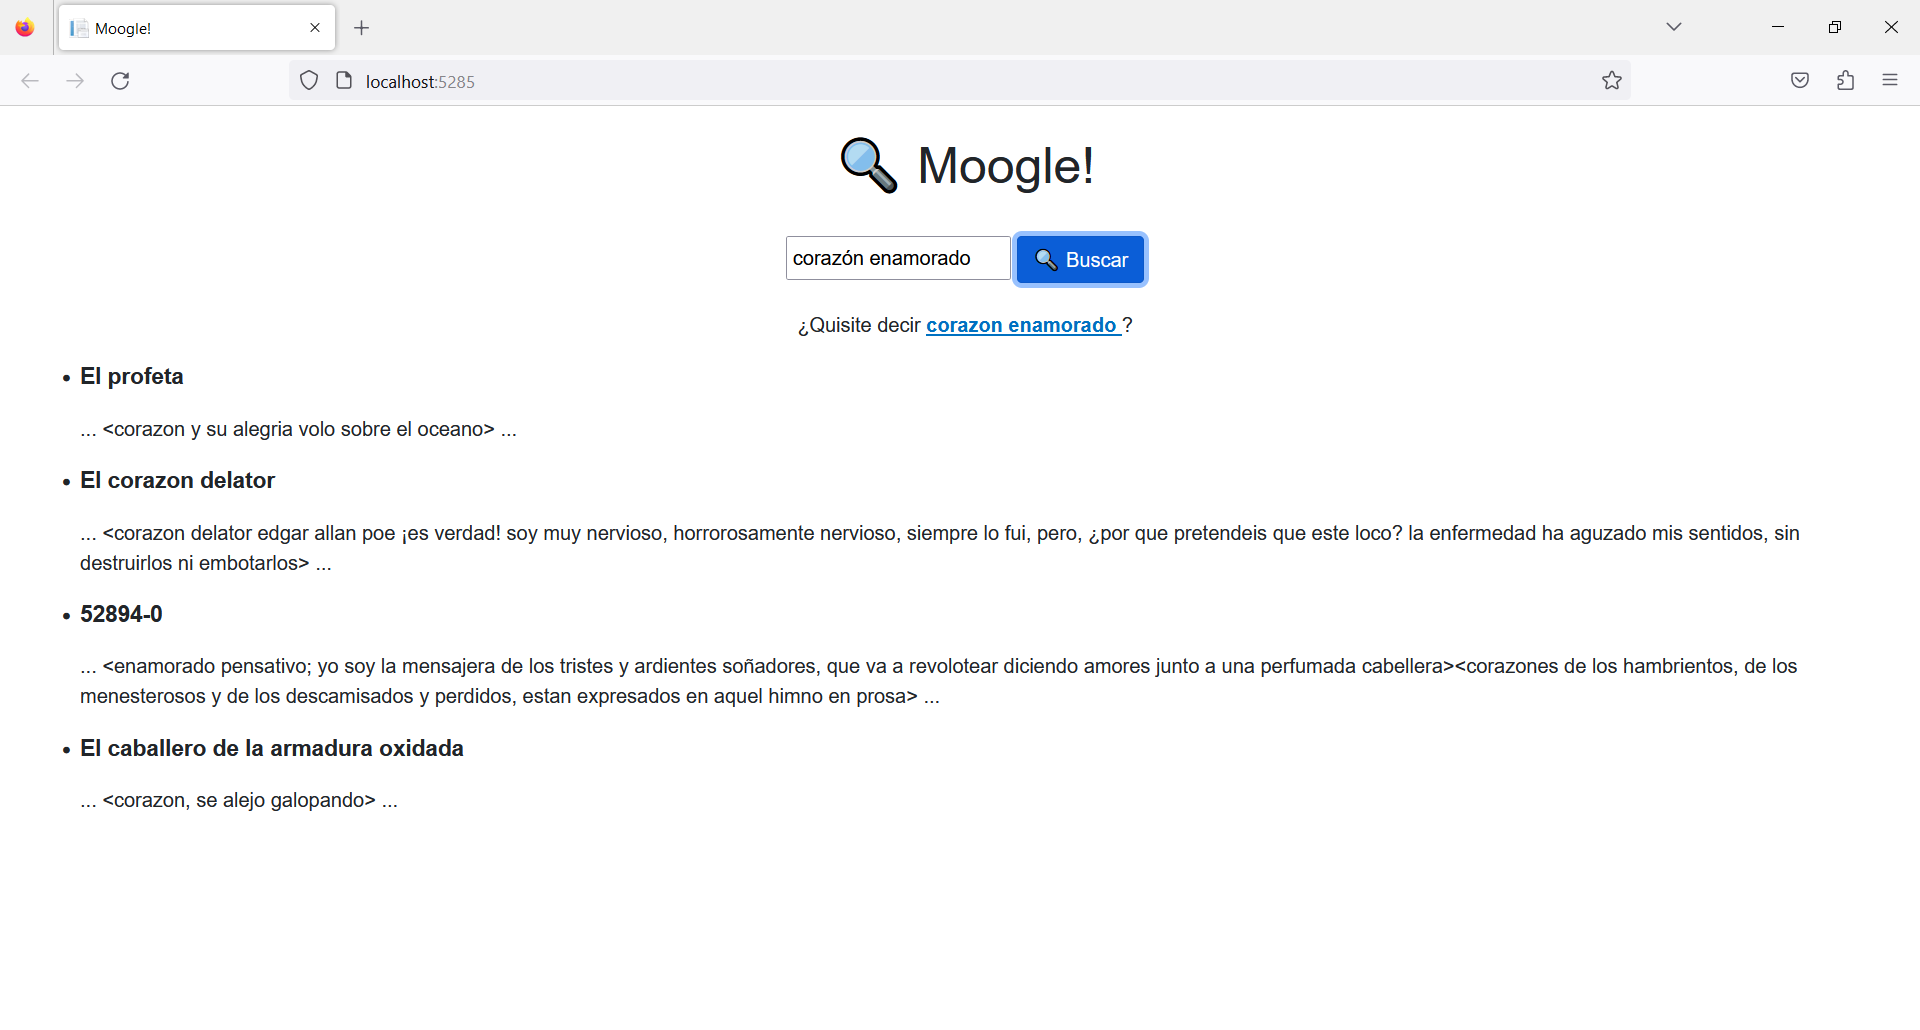
\includegraphics[scale=0.24]{img3.png}
			\caption{Resultados de la búsqueda}
			\label{fig: Figura 3}
		\end{figure}
	\end{frame}
	
	\begin{frame}{¿Cómo trabajar con esta aplicación?}
		Si cuando se escribe el texto de búsqueda contiene alguna palabra mal escrita o que no existe en los ficheros que se tienen predeterminados, el sistema mostrará una sugerencia.
	
	\begin{figure}[H]
		\centering
		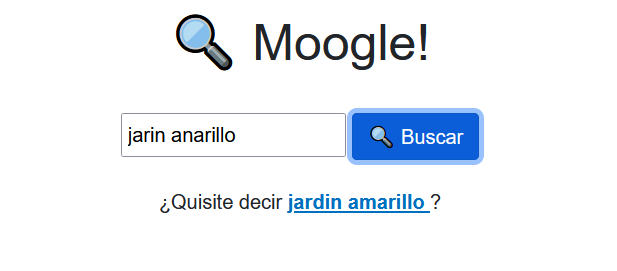
\includegraphics[scale=0.5]{img4.png}
		\caption{Sugerencia}
		\label{fig: Figura 4}
	\end{figure}
	\end{frame}
	
	\begin{frame}
		\justifying
		Se puede entonces presionar con el mouse sobre la sugerencia (el texto subrayado y en azul) y entonces el sistema vuelve a hacer la búsqueda, ahora con dicho texto.
		
		\begin{figure}[H]
			\centering
			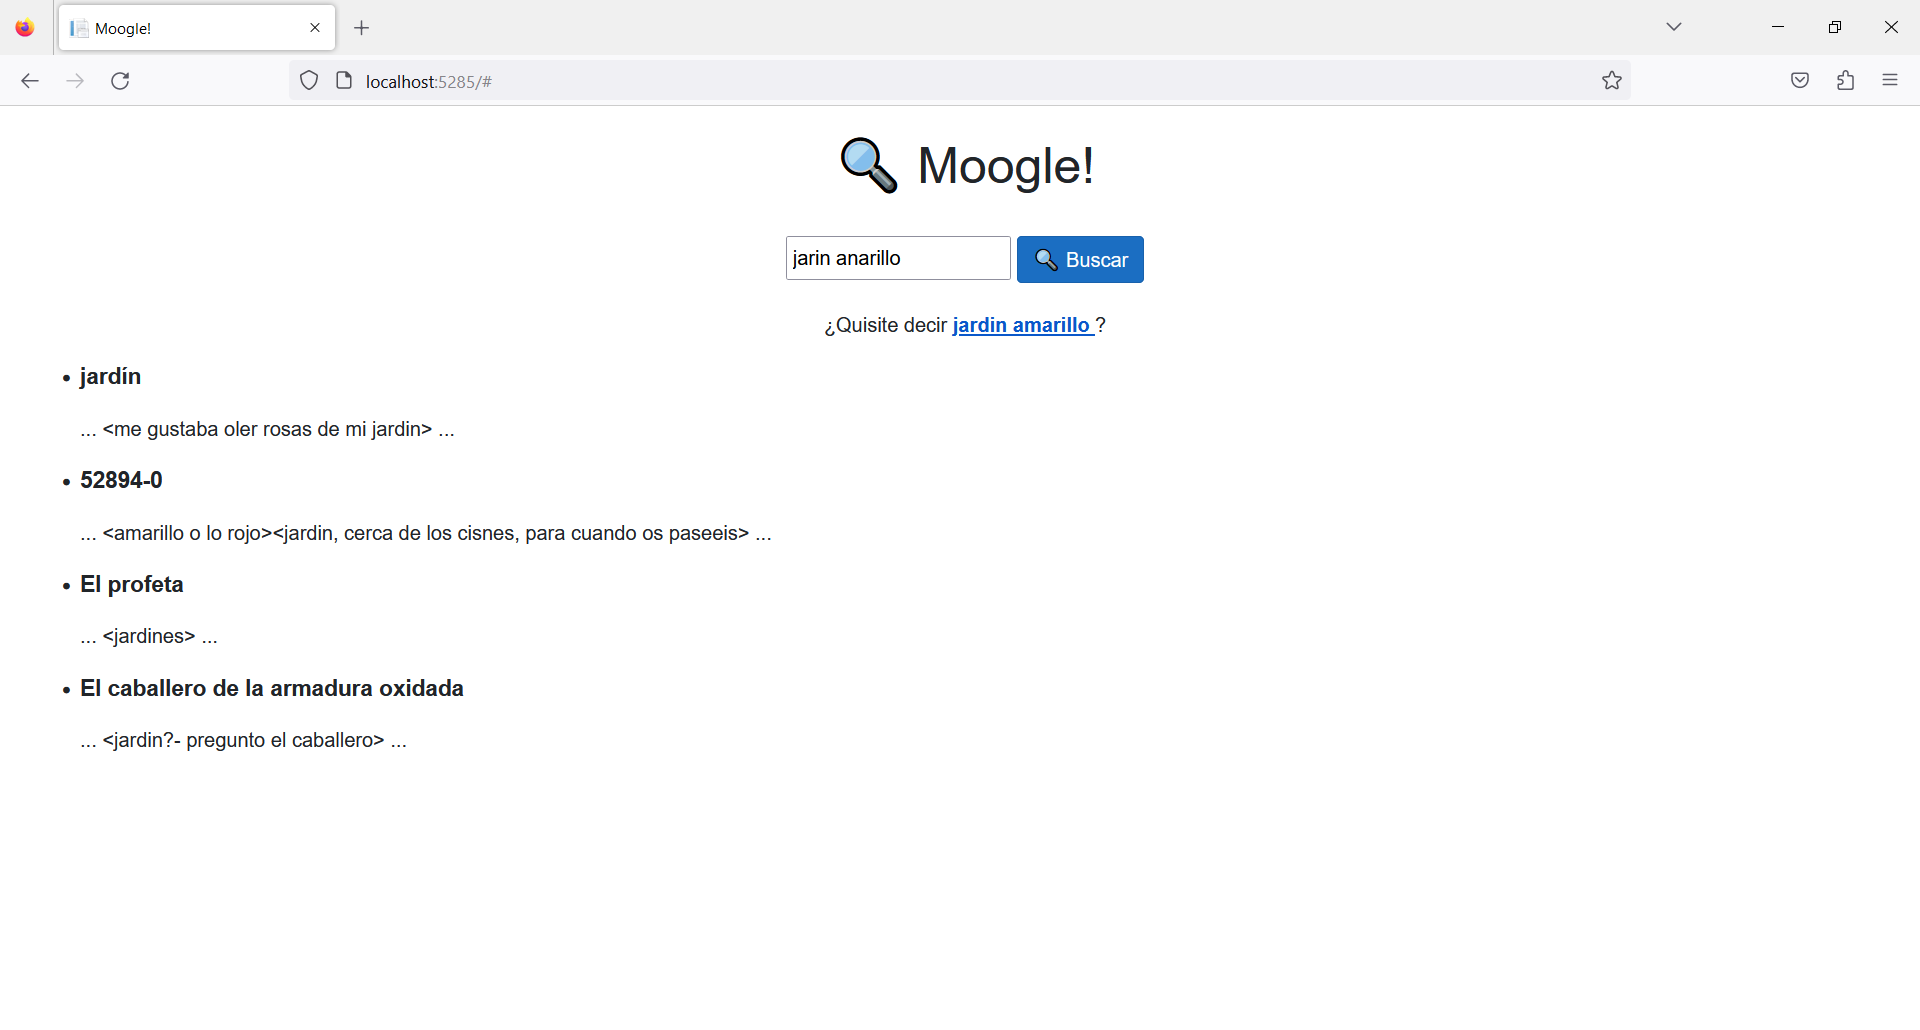
\includegraphics[scale=0.22]{img5.png}
			\caption{Repetir proceso de generar la sugerencia}
			\label{fig: Figura 5}
		\end{figure}
	\end{frame}
	
	\section {Características del desarrollo del trabajo}
	\begin{frame}{Características del desarrollo del trabajo}
		\justifying
		Para lograr este desempeño del sistema, hubo que realizar un trabajo de desarrollo y codificación. Las características de este desarrollo son las siguientes:
		
		\begin{enumerate}
			\item Primero se guarda en una variable el directorio actual sobre el que se está ejecutando el aplicativo, y en ese camino es donde se encuentra la carpeta Content que es la que contiene los ficheros .txt sobre los cuáles se realizará la búsqueda.
			
			\item[2.] Estos ficheros se leen y se guardan en un arreglo.
			
			\item[3.] Se recorre este arreglo y fichero a fichero se guarda el contenido del mismo en un string. 
		\end{enumerate}
	\end{frame}
	
	\begin{frame}{Características del desarrollo del trabajo}
		
		\begin{enumerate}
			\item[4.] Ese string se convierte a minúscula y se normaliza (se le quitan los acentos, caracteres especiales, espacios en blanco, signos de puntuación, etc) y se separa por palabras, las cuáles se guardan en un arreglo.
			Los métodos que leen el contenido del fichero y lo normalizan se encuentran en la clase Document.
			
			\item[5.] Después se recorre este arreglo palabra a palabra y se va contando la cantidad de veces que aparecen en el texto y se guarda en un diccionario dicha relación.
			A su vez estos diccionarios que se van creando por cada fichero se insertan en una lista.
		\end{enumerate}
	\end{frame}
	
	\begin{frame}{Características del desarrollo del trabajo}
		\begin{enumerate}
			
			\item[6.] Posteriormente se crea la matriz TFIDF con los pesos de las palabras de cada fichero. 
			Para esto se crea la clase TFidfCalculator que contiene los métodos para calcular los parámetros que son necesarios para llevar a cabo los cálculos de los pesos para poder llenar la matriz, la cuál se llena también dentro de esta clase a partir de un método desarrollado para ello.
			
			\item[7.] Después con la query se hace algo similar.
			Se crea un diccionario donde se guardan las palabras de la query y la cantidad de veces que aparecen en la misma.
			
			\item[8.] Se calcula entonces el peso de las palabras de la query y se llena otro diccionario con dicha información.
			
		\end{enumerate}
	\end{frame}
	
	\begin{frame}{Características del desarrollo del trabajo}
		\begin{enumerate}
			
			\item[9.] A continuación, se recorre la matriz que contiene los pesos de las palabras de los documentos y junto con los pesos de las palabras de la query se calcula a partir de la fórmula de similitud de coseno, el score de cada palabra.
			Con esta información se llena un diccionario que tiene como llave los documentos y como valor su correspondiente score.
			
			\item[10.] Para poder devolver los ficheros que más alto score poseen, se ordena este diccionario descendentemente. Se recorren entonces los cinco ficheros de más alto score, que son los que se van a mostrar.
			
			\item[11.] De estos ficheros se recorren cada una de sus palabras ordenadas descendentemente por su peso y se trabaja con aquellas que tienen peso superior a 20 (cálculo estimado que permite desestimar las palabras sin interés como los artículos, preposiciones y otras)
		\end{enumerate}
	\end{frame}
	
	\begin{frame}{Características del desarrollo del trabajo}
		\begin{enumerate}
			
			\item[12.] Se buscan estas palabras en el texto del fichero y se devuelve un fragmento del mismo (o snippet). Para esto se toma el texto desde dónde aparece dicha palabra hasta el punto más cercano a la misma.
			
			\item[13.] Por último, se desarrolló lo referente a la sugerencia. Para esto se creó una clase CrearSugerencia que contiene un método que obtiene la palabra que más se asemeja a la entrada por el usuario. 
			Esto lo hace recorriendo la lista de todas las palabras que existen en todos los ficheros, y comparando cada letra de estas palabras con cada letra de la palabra entrada por el usuario. Si no coincide la letra pues busca cuál sería la palabra con menor distancia (menos cambios de letras) y esa es la que debería ser la más similar y es entonces la que se devuelve.
		\end{enumerate}
	\end{frame}
\end{document}